%\begin{frame}{Our NKM in the general deterministic framework}
%	\begin{wideitemize}
%	\item General deterministic model: $f\left(x_{t-1},x_t,x_{t+1},u_t | \theta \right)$
%	    \item Our model:
%	    \begin{align*}
%	        x_t &= \left(\pi_t \quad y_t \quad i_t \quad \cdots\right)'\\
%	           u_t &= \left(u^a_t \quad u^c_t \quad  u^i_t\right)'
%	    \end{align*}
%        \item Thus (omitting the shock processes):
%       \begin{align*}
%        f\left(x_{t-1},x_t,x_{t+1},u_t | \theta \right) =
%            \begin{pmatrix}
%                \pi_t - \beta E_t\left[\pi_{t+1}\right]-\kappa y_t- \varepsilon_t^a  \\
%                y_t -E_t \left[y_{t+1} \right]+ \frac{1}{\sigma}\left(i_t-E_t\left[\pi_{t+1}\right]\right)-\varepsilon_t^c  \\
%                i_t - \phi_\pi \pi_t - \phi_y y_t-\varepsilon_t^i \\
%                \vdots
%            \end{pmatrix}
%        \end{align*}
%    \end{wideitemize}
%\end{frame}
%
%
%\begin{frame}{Model solution: Stacked system}
%    \begin{wideitemize}
%    \item Dynare solves a stacked system of nonlinear difference equations:\footnote{\url{https://stephane-adjemian.fr/dynare/slides/perfect-foresight-models.pdf}}
%    \begin{align*}
%    f\left(x_{2},x_{1},{\color{red}x_{0}},u_{1}\right) &= 0\\
%    f\left(x_{3},x_{2},x_{1},u_{2}\right) &= 0\\
%    \vdots \\
%    f\left(x_{t+1},x_{t},x_{t-1},u_{t}\right) &= 0\\
%    \vdots \\
%    f\left({\color{red}x_{T+1}},x_{T},x_{T},u_{T}\right) &= 0
%    \end{align*}
%    \item Compact notation: $F\left(\boldsymbol{X}\right) = 0$ with $\boldsymbol{X} = [x_1',x_2',...,x_T']'$, i.e. the entire solution path.
%    \item Boundary conditions: $x_0$ and $x_{T+1}$
%    \end{wideitemize}
%\end{frame}
%
%\begin{frame}{Numerical approach: Newton algorithm}
%\begin{columns}
%    \begin{column}[T]{0.8\textwidth}
%	    \begin{itemize}
%	        \item Start an initial guess $\boldsymbol{X^{(0)}}$
%	        \item Update the trajectories (solution paths) by iterating ($i = 0.1,...$) and solving:
%	        \begin{equation*}
%	           F\left(\boldsymbol{X}^{i+1}\right) =   J_F\left(\boldsymbol{X}^{i+1}\right)\left( \boldsymbol{X}^{(i+1)}-\boldsymbol{X}^{(i)}\right)
%	        \end{equation*}
%	        where $J_F\left(\boldsymbol{X}^{i+1}\right)$ is the Jacobian matrix of partial derivatives of $F()$.
%	        \item Stop if
%	         \begin{equation*}
%	           || F\left(\boldsymbol{X}^{i+1}\right) || < crit.
%	        \end{equation*}
%	        \item Lot's of room for improvement:
%	        \begin{itemize}
%    	        \item The size of $J_F$: Exploit sparsity and triangular model structure.
%    	       \item Optimise step size
%	        \end{itemize}
%	    \end{itemize}
%\end{column}
%\begin{column}[T]{0.2\textwidth}
%
%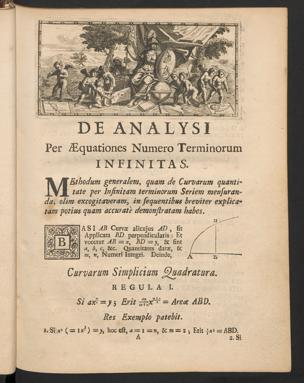
\includegraphics[width=1\textwidth]{figures/newton.jpg}\\
% \href{https://de.wikipedia.org/wiki/Datei:NewtonIteration_Ani.gif}{Link to a simple example.}
%\end{column}
%\end{columns}
%\end{frame}
%
%\begin{frame}{Deterministic simulation in Dynare}
%Keywords:
%    \begin{wideitemize}
%    \item \texttt{initval}: Sets the initial steady state
%    \item \texttt{endval}: Sets the terminal steady state
%    \item \texttt{shocks}: Specify shocks for the simulation path
%    \item \texttt{histval}: For states outside the steady state
%    \item \texttt{perfect\_foresight\_setup}; sets up the simulation
%    \item \texttt{perfect\_foresight\_solver}; run the simulations
%    \item Many options are available. See the Dynare manual.
%    \end{wideitemize}
%\end{frame}

\begin{frame}[fragile]{Perfect foresight: brute force ELB implementation}
\begin{wideitemize}
\item ELB implementation via $\max$-operator in the \texttt{model}-block.
\begin{minted}{c++}
[name='Notional rate Taylor rule']
inomnot=rhoinom*inomnot(-1)
        +(1-rhoinom)*(phi_pi*pie+phi_y*y)+zeps_i;

[name = 'Observed interest rate']
inom = max(inomnot,ilb);
\end{minted}
\item Of note: $\max$-operator is not differentiable\\
$\rightarrow$ challenging for Newton-type solvers that rely on (sparse) Jacobian
\end{wideitemize}
\end{frame}


\begin{frame}[fragile]{Simulating a demand shock of 1\%}
\begin{minted}{c++}
shockssequence = -0.01;

shocks;
    var u_c;
    periods 1;
    values(shockssequence);
end;

perfect_foresight_setup(periods=50);
perfect_foresight_solver;
\end{minted}
\begin{wideitemize}
\item Important: allow for sufficiently many periods to return back to steady state
\end{wideitemize}
\end{frame}


\begin{frame}[fragile]{Perfect foresight: mixed complementarity problem (MCP) implementation}
\begin{wideitemize}
\item Alternative: use specialized \hi{mixed complementary problem (MCP)} solver:
\begin{itemize}
\item Levenberg-Marquardt mixed complementarity problem solver \parencite{KanzowPetra2004} triggered by keyword \texttt{lmmcp} or\\
     \texttt{perfect\_foresight\_solver(stack\_solve\_algo=7, solve\_algo=10)}
\item PATH solver \parencite{FerrisMunson1999}: \\ \texttt{perfect\_foresight\_solver(stack\_solve\_algo=7, solve\_algo=11)}
\end{itemize}
\item Solvers require particular type of setup:
\begin{align}
        LB =&X  &\Rightarrow   F(X)>0,\\
       LB\leq &X \leq UB &\Rightarrow   F(X)=0,\\
        &X =UB &\Rightarrow   F(X)<0.
\end{align}
\item Sign of the equation residual with binding constraint matters
\item Convention in Dynare: LHS-RHS
\end{wideitemize}
\end{frame}

\begin{frame}[fragile]{Perfect foresight: MCP implementation}
\begin{wideitemize}
\item Explicitly specify a complementarity condition for the Taylor rule using the perpendicular symbol:
\begin{itemize}
        \item  ⟂ UTF-8 symbol (Unicode codepoint U+27C2)
        \item  \textunderscore|\textunderscore : pure ASCII, i.e. a vertical bar enclosed within two underscores
\end{itemize}
\begin{minted}{c++}
[name='Notional rate Taylor rule'] 
inom=inomnot ⟂ inom>-0.0055;

[name='Notional rate Taylor rule']
inomnot=rhoinom*inomnot(-1)
        +(1-rhoinom)*(phi_pi*pie+phi_y*y)+zeps_i;
\end{minted}
\item If lower bound on interest rate is binding
\begin{equation}
  residual=i_t-i_t^{not}>0
\end{equation}

\end{wideitemize}
\end{frame}

\begin{frame}[fragile]{Perfect foresight: MCP implementation}
\begin{wideitemize}
\item Alternative: older syntax where \texttt{mcp}-tag indicates equation to be replaced (RHS expression is not parsed!)
\begin{minted}{c++}
[name='Notional rate Taylor rule',mcp='inom>-0.0055']
inom=inomnot;

[name='Notional rate Taylor rule']
inomnot=rhoinom*inomnot(-1)
        +(1-rhoinom)*(phi_pi*pie+phi_y*y)+zeps_i;
\end{minted}
\item If lower bound on interest rate is binding
\begin{equation}
  residual=i_t-i_t^{not}>0
\end{equation}

\end{wideitemize}
\end{frame}


\begin{frame}[fragile]{Simulating a demand shock of 1\%}
\begin{minted}{c++}
shockssequence = -0.01;

shocks;
    var u_c;
    periods 1;
    values(shockssequence);
end;

perfect_foresight_setup(periods=50);
perfect_foresight_solver(lmmcp);
\end{minted}
\begin{itemize}
\item Specialized solver triggered by keyword \texttt{lmmcp}
\end{itemize}
\end{frame}

%\begin{frame}[fragile]{Pre-announced shock}
%\begin{wideitemize}
%\item Example of a pre-announced monetary policy shock
%\begin{minted}{c++}
%shockssequence = 0.01;
%
%shocks;
%var u_i;
%periods 4;
%values(shockssequence);
%end;
%
%perfect_foresight_setup(periods=300);
%perfect_foresight_solver;
%\end{minted}
%\end{wideitemize}
%\end{frame}
%
%
%
%
%\begin{frame}[fragile]{Permanent shock}
%\begin{wideitemize}
%\item Example of a permanent cost-push shock
%\begin{minted}{c++}
%initval;
%u_a = 0;
%end;
%steady ;
%
%endval;
%u_a = -0.001;
%end;
%steady;
%
%perfect_foresight_setup(periods=300);
%perfect_foresight_solver;
%\end{minted}
%\end{wideitemize}
%\end{frame}



%\begin{frame}[fragile]{Output}
%\begin{wideitemize}
%\item Dynare stores the endogenous variables $\left(x_0 \quad x_1  \quad ... x_T \quad x_{T+1}\right)$ in the field \texttt{oo\_.endo\_simul}
%\item Dynare stores the exgenous variables $\left(u_1  \quad ... u_T \right)'$ in the field \texttt{oo\_.exo\_simul}
%\end{wideitemize}
%\end{frame}
%
%
%
%\begin{frame}{Hands-on}
%\begin{wideitemize}
%\item Let's look at the \hi{code for deterministic simulations} in practice.
%\end{wideitemize}
%\end{frame} 